

\begin{figure}[h!]
	\centering
 	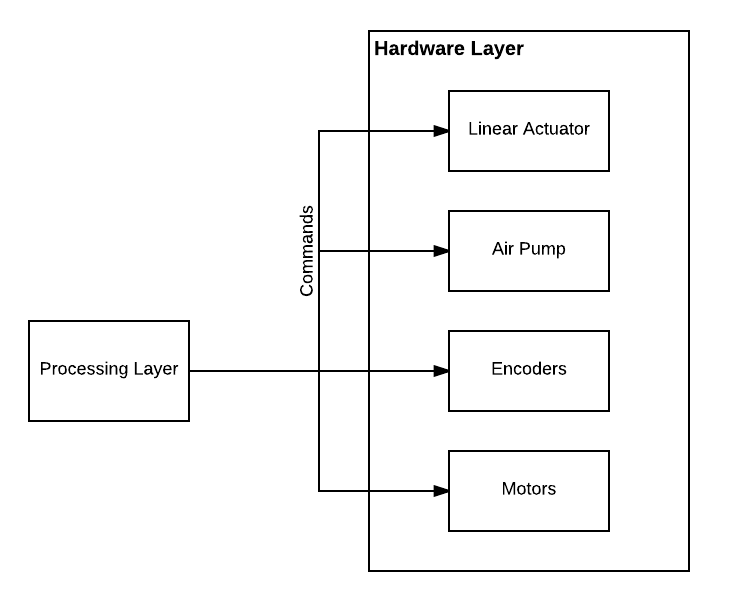
\includegraphics[width=0.60\textwidth]{images/hardware}
 \caption{Hardware Layer subsystem diagram}
\end{figure}

\subsection{Linear Actuator Subsystem}
The linear actuator is what moves the end effector down and up in order to grip an object

\subsubsection{Assumptions}
The subsystem will be able to receive commands in order to know when to operate its movement

\subsubsection{Responsibilities}
This subsystem is responsible for receiving its commands and making its movements when it should in a timely manner.

\subsubsection{Subsystem Interfaces}


\begin {table}[H]
\caption {Linear Actuator interfaces} 
\begin{center}
    \begin{tabular}{ | p{1cm} | p{6cm} | p{3cm} | p{3cm} |}
    \hline
    ID & Description & Inputs & Outputs \\ \hline
    \#1 & Command Data from Teensy & \pbox{3cm}{Commands} & \pbox{3cm}{Actuator movement}  \\ \hline

    \end{tabular}
\end{center}
\end{table}

\subsection{Motor Step Movement Subsystem}
The Stepper Motors are what moves the joints of the robot arm.

\subsubsection{Assumptions}
The subsystem will be able to receive commands in order to know when to operate its movement

\subsubsection{Responsibilities}
This subsystem is responsible for receiving its commands and making its movements when it should in a timely manner.

\subsubsection{Subsystem Interfaces}


\begin {table}[H]
\caption {Motor interfaces} 
\begin{center}
    \begin{tabular}{ | p{1cm} | p{6cm} | p{3cm} | p{3cm} |}
    \hline
    ID & Description & Inputs & Outputs \\ \hline
    \#1 & Command Data from Teensy & \pbox{3cm}{Commands} & \pbox{3cm}{Motor movement}  \\ \hline

    \end{tabular}
\end{center}
\end{table}

\subsection{Encoder Position Subsystem}
The Encoder subsystem should be able to take the angle of the arm joints and communicate the angle positions in order to provide motion control.

\subsubsection{Assumptions}
The subsystem will be able to receive commands in order to know when to operate its control

\subsubsection{Responsibilities}
This subsystem is responsible for receiving its commands and controling the movement accurately.

\subsubsection{Subsystem Interfaces}


\begin {table}[H]
\caption {Encoder interfaces} 
\begin{center}
    \begin{tabular}{ | p{1cm} | p{6cm} | p{3cm} | p{3cm} |}
    \hline
    ID & Description & Inputs & Outputs \\ \hline
    \#1 & Command Data from Teensy & \pbox{3cm}{Commands} & \pbox{3cm}{Encoder Position}  \\ \hline

    \end{tabular}
\end{center}
\end{table}

\subsection{Air Pump Subsystem}
This subsystem receives commands to operate the vacuum air pump which manipulates the gripper and allows the gripper to hold onto objects.

\subsubsection{Assumptions}
The subsystem will be able to receive commands in order to know when to operate vacuum.

\subsubsection{Responsibilities}
This subsystem is responsible for receiving its commands and operating when it should in a timely manner.

\subsubsection{Subsystem Interfaces}


\begin {table}[H]
\caption {Air Pump interfaces} 
\begin{center}
    \begin{tabular}{ | p{1cm} | p{6cm} | p{3cm} | p{3cm} |}
    \hline
    ID & Description & Inputs & Outputs \\ \hline
    \#1 & Command Data from Teensy & \pbox{3cm}{Commands} & \pbox{3cm}{Air pump operation}  \\ \hline

    \end{tabular}
\end{center}
\end{table}